
\subsection{Explicación detallada del algoritmo}

En la sección anterior analizamos varios algoritmos de búsqueda local.
La búsqueda local es una heurística para algoritmos aproximados.
Sin embargo, las heurísticas de búsqueda local pueden verse como un algoritmo de \emph{gradient descent}.
Estos algoritmos tienen el problema de los mínimos locales: cuando encuentran un mínimo local se quedan trabados y no pueden mejorar esa solución no óptima. 

Por esa razón surgen las metaheurísticas.
Una metaheurística es un método heurístico para resolver un  problema computacional general.
Una meteheurística usa los parámetros dados por el usuario sobre unos procedimientos genéricos y abstractos. 
Normalmente, estos procedimientos son heurísticos.

En particular, nosotros utilizaremos la metaheurística del tabu search, que a su vez se basa en la heurística de búsqueda local.
Una explicación completa de la heurística de tabú search puede encontrarse en \cite{tabusearch}.

Expliquemos los detalles de nuestra implementación antes de ver el pseudocódigo.

Nuestra lista tabú en nuestro caso debería contener soluciones posibles, es decir, isomorfismos. Sin embargo, como comparar isomorfismos es muy caro, decidimos usar una función de hash y almacenar este valor. De esta manera, buscar soluciones en la lista tabú se vuelve mucho menos costoso.

Nuestra función de aspiración, es decir, nuestro método para elegir el isomorfismo inicial de la siguiente iteración hace lo obvio si hay alguna solución no tabú: elige la mejor.
Sin embargo, si todas las soluciones son tabú, elegiremos la mejor solución tabú en cuestión.

No creemos que fuera adecuado elegir ningún \emph{movimiento prohibido}, como vimos en la teórica (la definición de movimiento prohibido no existe en la definición original de la metaheuristica tabu search, si no que es una adición posterior), dado que no parecía razonable prohibir ningún movimiento ni ninguna solución particular (más allá de la tabú).
Esto se debe principalmente a que no hay características que hagan que, inmediatamente, podamos descartar una solución y declararla inviable.

Sin más que explicar, veamos nuestra implementación.


\begin{algorithm}[H]
  \begin{algorithmic}[1]
  \caption{Pseudocódigo del procedimiento Tabu Search}
  \label{algo:6-1}
    \Procedure{tabu\_search}
              {\texttt{Grafo} $g1$,
               \texttt{vector<int>} $vertices1$,
               \texttt{Grafo} $g2$,
               \texttt{vector<int>} $vertices2$} 
    \State $source \gets goloso(g1, vertices1, g2, vertices2)$
    \State $lista\_tabu \gets lista(1000, make\_pair(0, 0))$
    \State $indice\_lista\_tabu \gets 0$
    \State Inicializar estructuras relacionadas con el criterio de parada.
    \While {criterio de parada} 
       \State $mejor\_tabu \gets \{.isomorfismo = Isomorfismo(), .aristas = 0\}$
       \State $mejor\_solucion \gets \{.isomorfismo = Isomorfismo(), .aristas = 0\}$
       \For $vecino \in vecindad(source)$
           \State $aristas \gets buscar(lista_tabu, hash(vecino))$
           \If {$aristas = 0$}
               \Comment Source es una solución tabu.
               \If {$aristas > mejor\_tabu.aristas$}
                   \State $mejor\_tabu.aristas \gets aristas$
                   \State $mejor\_tabu.isomorfismo \gets vecino$
                   \State continue
               \EndIf
           \Else
               \State $aristas = contar\_aristas\_isomorfismo(g1, g2, vecino)$
               \If {$aristas > mejor\_tabu.aristas$}
                   \State $mejor\_solucion.aristas \gets aristas$
                   \State $mejor\_solucion.isomorfismo \gets vecino$
                   \State continue
               \EndIf
           \EndIf
        \EndFor
        \If {$mejor\_solucion.aristas > 0$}
            \State $lista\_tabu.push\_back($
            \State \,\,  $make\_pair(
              hash(mejor\_solucion.isomorfismo),
              mejor\_solucion.aristas))$
            \If {$lista\_tabu.size() > lista\_tabu\_limite$}
                 \State $lista\_tabu.pop\_front()$
            \EndIf
        \EndIf
        \If {$mejor\_solucion.aristas = 0$}
           \Comment Todas las soluciones son tabu.
           \State $source \gets mejor\_tabu$
       \Else
           \State $source \gets mejor\_solucion$
       \EndIf
       \State Actualizar estructuras relacionadas con el criterio de parada.
    \EndWhile
           
		\EndProcedure
	\end{algorithmic}
\end{algorithm}


Para la experimentación, decidimos plantear tres tamaños distintos de lista tabú.
A continuación, detallaremos nuestras expectativas.
El tamaño más pequeño funcionará muy rápido, dado que la búsqueda es muy efectiva, pero la calidad de los resultados será la peor de entre todas, dado que no podremos guardar muchos resultados previos.
El tamaño más grande nos proveerá de los mejores resultados (en promedio) pero la búsqueda en la lista será terriblemente lenta, por lo cual no valdrá tanto la pena.
El tamaño intermedio será, según nuestra creencia, un balance entre velocidad y calidad de los resultados.

En cuanto a los criterios de parada, hay varios de entre los cuales elegir, pero todos se reducen a los mismos dos criterios de parada. Analic\'emoslos.

\begin{enumerate}
  \item Primero, podemos setear una cantidad de iteraciones global $k$, y simplemente parar luego de que la cantidad de iteraciones supera $k$. Este es el criterio más simple y esperamos que funcione peor que el siguiente.
  \item El segundo criterio de parada, es un criterio que se fija cuantas iteraciones pasaron desde que la solución fue mejorada por última vez. Una vez que esa cantidad de iteraciones supera un límite $k$, el algoritmo terminará.
\end{enumerate}

Esperamos que el segundo criterio funcione mucho mejor, dado que se adapta a lo que esta sucediendo en cada momento: si encuentra cada vez mejores soluciones sigue buscando y si deja de encontrar mejores soluciones termina. Sin embargo, lo bueno del otro criterio de parada, es que tenemos asegurado que va a terminar dentro de un margen de tiempo que podemos determinar muy fácilmente con el límite de iteraciones $k$.





\subsection{Performance del algoritmo}


Para testear tanto este algoritmo como las heurísticas, utilizamos los casos cuya generación está explicada en el ap\'endice.

Antes de empezar con la explicación, debemos comentar que los tests de calidad y tiempos del tabú search son muy intensos computacionalmente: debían ser corridos por varias horas para que terminen.

Lo que presentamos es el resultado final, que aunque es el resultado de una sola corrida de varias horas, necesito algunas decenas de intentos anteriores, con el objetivo de encontrar los parámetros más interesantes a ser mostrados en el informe.

Por esa razón debimos limitar la cantidad de muestras que tomamos, lo cual, como vermos impactará un poco en las conclusiones que podremos obtener.
Sin embargo, los resultados son muy interesantes, y en el ejercicio 7 mostraremos algunos resultados que complementarán lo que no pudimos ver aquí.




En los gráficos, se verá que en el eje horizontal aparecen numeros de la pinta $n/m$.
$n$ será el criterio de parada utilizado, llamaremos 0 al criterio que cuenta la cantidad de iteraciones sin mejorar (el límite elegido será 500) y 1 al que harcodea el total de iteraciones (el límite elegido será 2000).
$m$ será el largo de la lista tabú.


Una aclaración importante es que probamos con distintos límites de iteraciones para cada criterio de parada y la diferencia en tiempo era la obvia (escalaba linealmente) y la diferencia en calidad era casi nula (a menos que las iteraciones fueran menores a 100. Por esa razón elegimos esas cantidades de iteraciones que nos parecieron lo suficientemente razonables.

No incluimos los gráficos de esos experimentos porque son mas que nada preliminares y no contribuyen a comparar las variantes, si no simplemente a optimizar los parámetros de cada una de ellas.



Primero analicemos la ``calidad'' de los algoritmos, es decir, que tan buenos son los resultados que devuelven. La métrica que utilizaremos es las aristas extra que devuelven, es decir, la cantidad de aristas que le agregan a la solución fuente, que es la de la heurística golosa.

Esta comparación será relativa: compararemos variantes del algoritmo unas contra otras, sin saber cual es la solución optima. Compararemos las soluciones del tabu search contra soluciones optimas en el ejercicio 7, aquí sólo nos atañe comparar las diferentes variantes de nuestro algoritmo.

Como dijimos anteriormente, la intensidad computacional de los algoritmos no permitió que podamos testear con grafos extremadamente grandes, utilizamos grafos de tamaño 150 como máximo. Sin embargo, 150 es un tamaño suficientemente grande, dado que ya a partir de 500, simplemente una corrida de un algoritmo comienza a tardar en el orden de 15 minutos: ni mencionar lo que se demora un test entero.

%% CALIDAD

\begin{figure}[H]
 \centering
	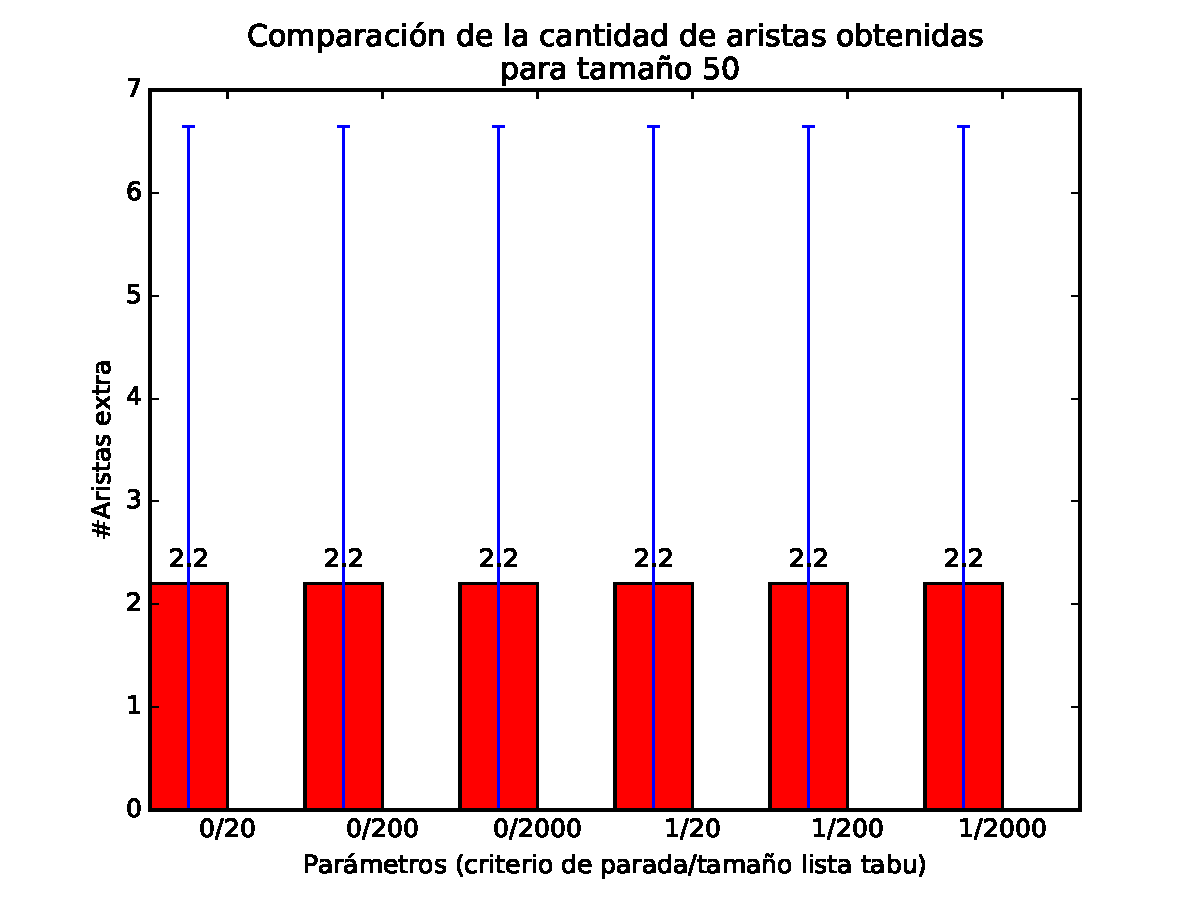
\includegraphics[width=0.8\textwidth]{graficos/problema_6/calidad0.pdf}
	\caption{}
	\label{fig:problema6-calidad0}
\end{figure}


\begin{figure}[H]
 \centering
	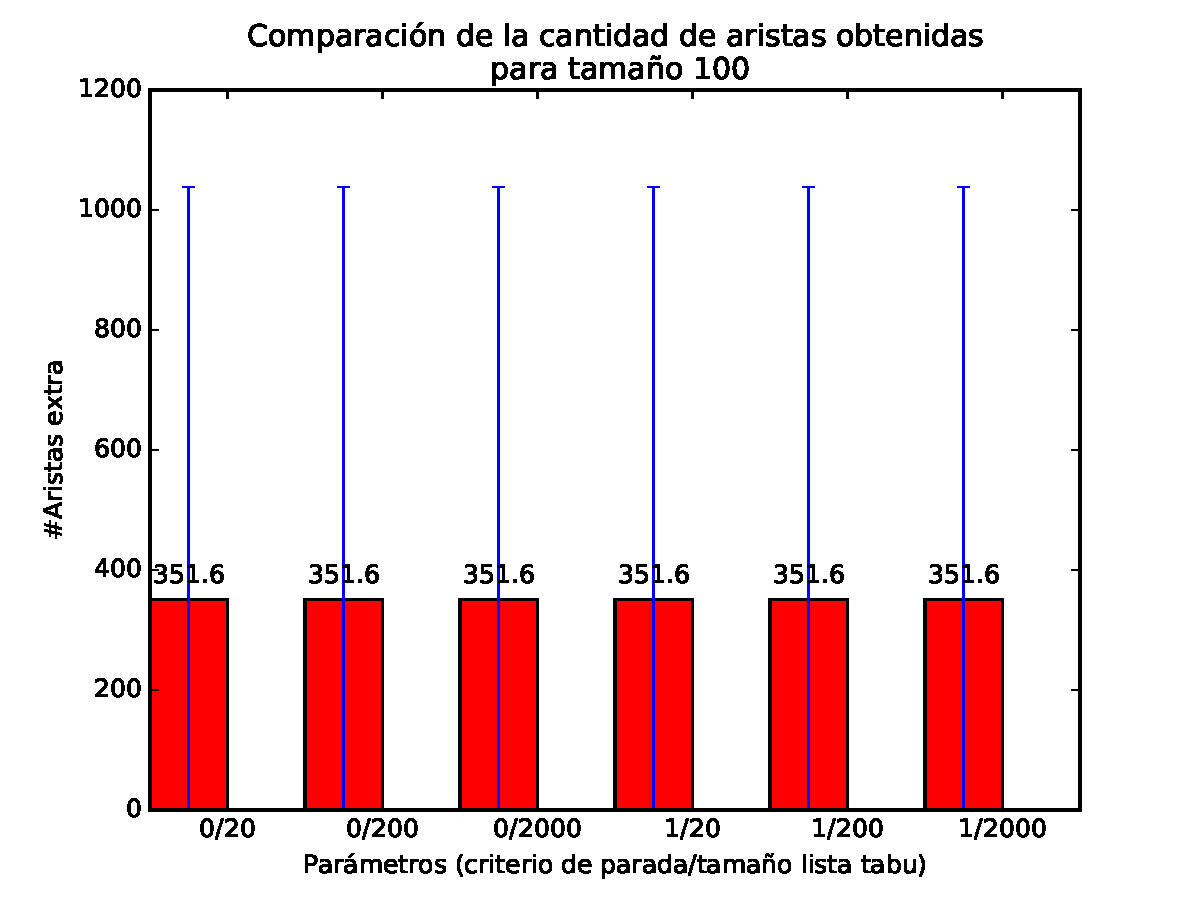
\includegraphics[width=0.8\textwidth]{graficos/problema_6/calidad1.pdf}
	\caption{}
	\label{fig:problema6-calidad1}
\end{figure}

\begin{figure}[H]
 \centering
	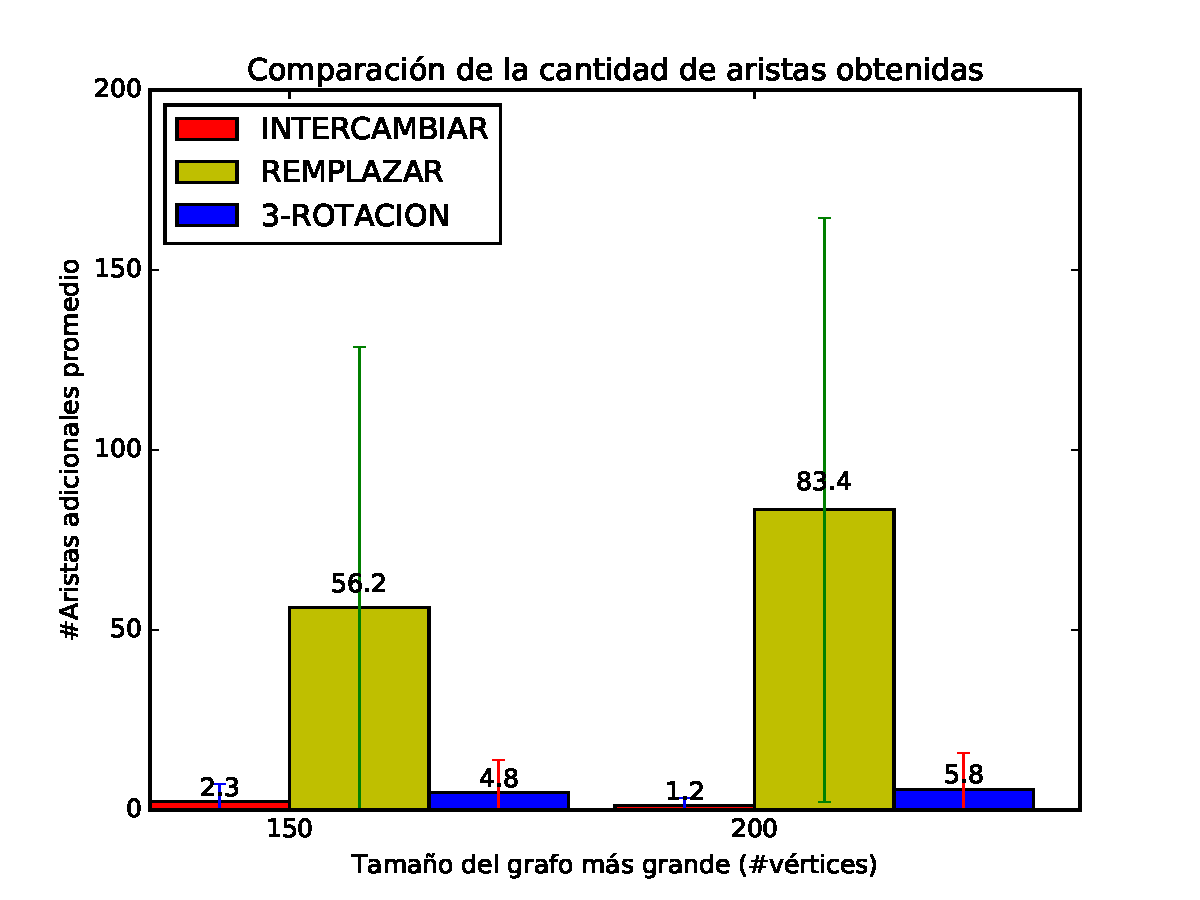
\includegraphics[width=0.8\textwidth]{graficos/problema_6/calidad2.pdf}
	\caption{}
	\label{fig:problema6-calidad2}
\end{figure}

En los gráficos se marca el promedio con una barra y la desviación estándar con un segmento.

Como podemos observar, no hay diferencia en el promedio de calidad de las mediciones.
Sin embargo, pudimos observar algunas diferencias en los máximos y los mínimos. Los mínimos de la variante que cuenta cuantas iteraciones no se mejoró eran mas altos.

Esto se debe a que el tamaño de los grafos no es lo suficientemente grande como para que dos algoritmos buenos hagan diferencia. Sin embargo, los grafos son lo suficientemente grandes como para asegurarnos que la diferencia entre las variantes no será demasiada en ningún caso (salvo casos patológicos).


A continuación, analizaremos los tiempos de los algoritmos. Nuestra expectativa, es que el tiempo que tarda la variante 0, es decir, la que fija la cantidad de iteraciones máxima sin que se mejore la solucion, va a ser mejor dado que optimiza la cantidad de iteraciones "ociosas", sobre todo en grafos chicos, donde la búsqueda se estanca relativamente rápido.

Además, esperamos que las variantes que tienen una lista tabú más larga tardan más, debido a que usamos una lista enlazada (std::list) para representarla, por lo que la búsqueda dentro de ella tiene complejidad lineal.

%% TIEMPOS
\begin{figure}[H]
 \centering
	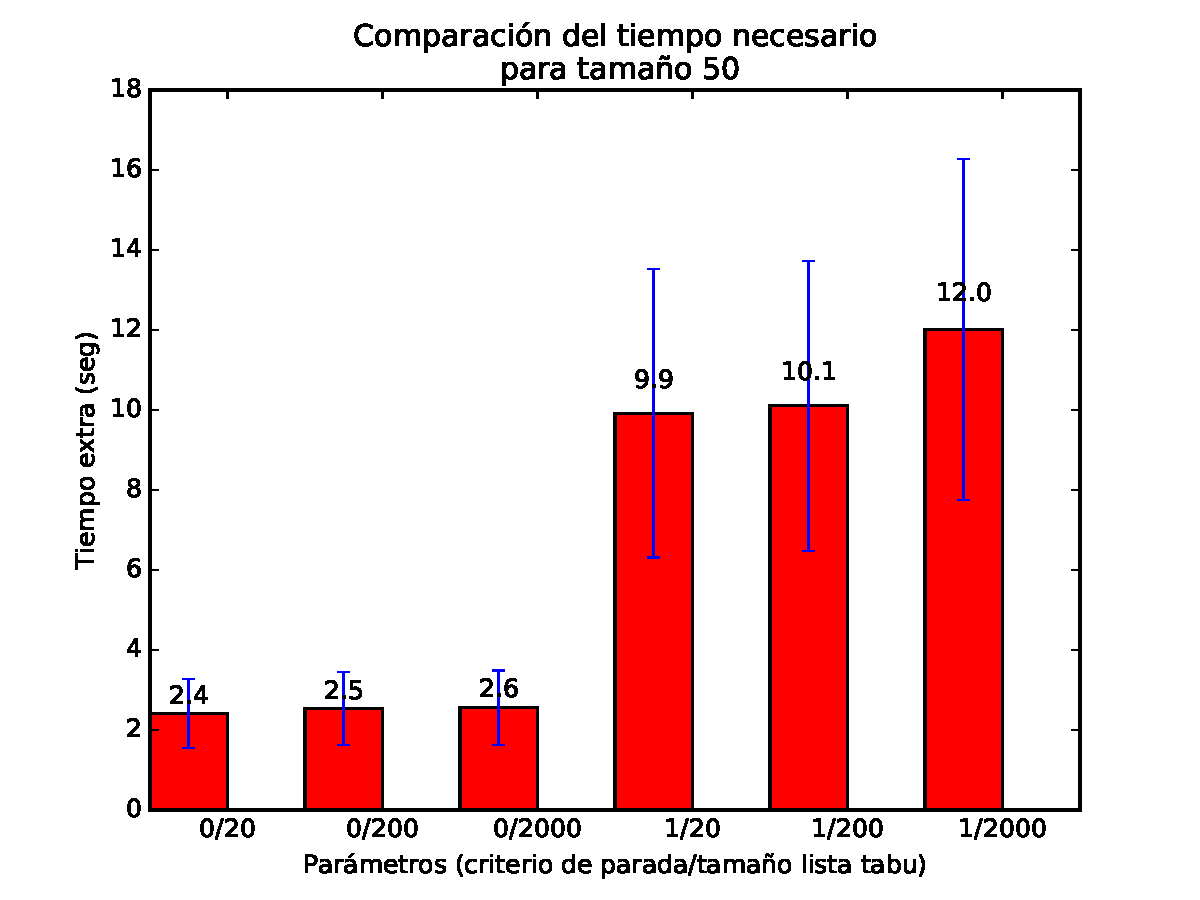
\includegraphics[width=0.8\textwidth]{graficos/problema_6/tiempo0.pdf}
	\caption{}
	\label{fig:problema6-tiempo0}
\end{figure}

\begin{figure}[H]
 \centering
	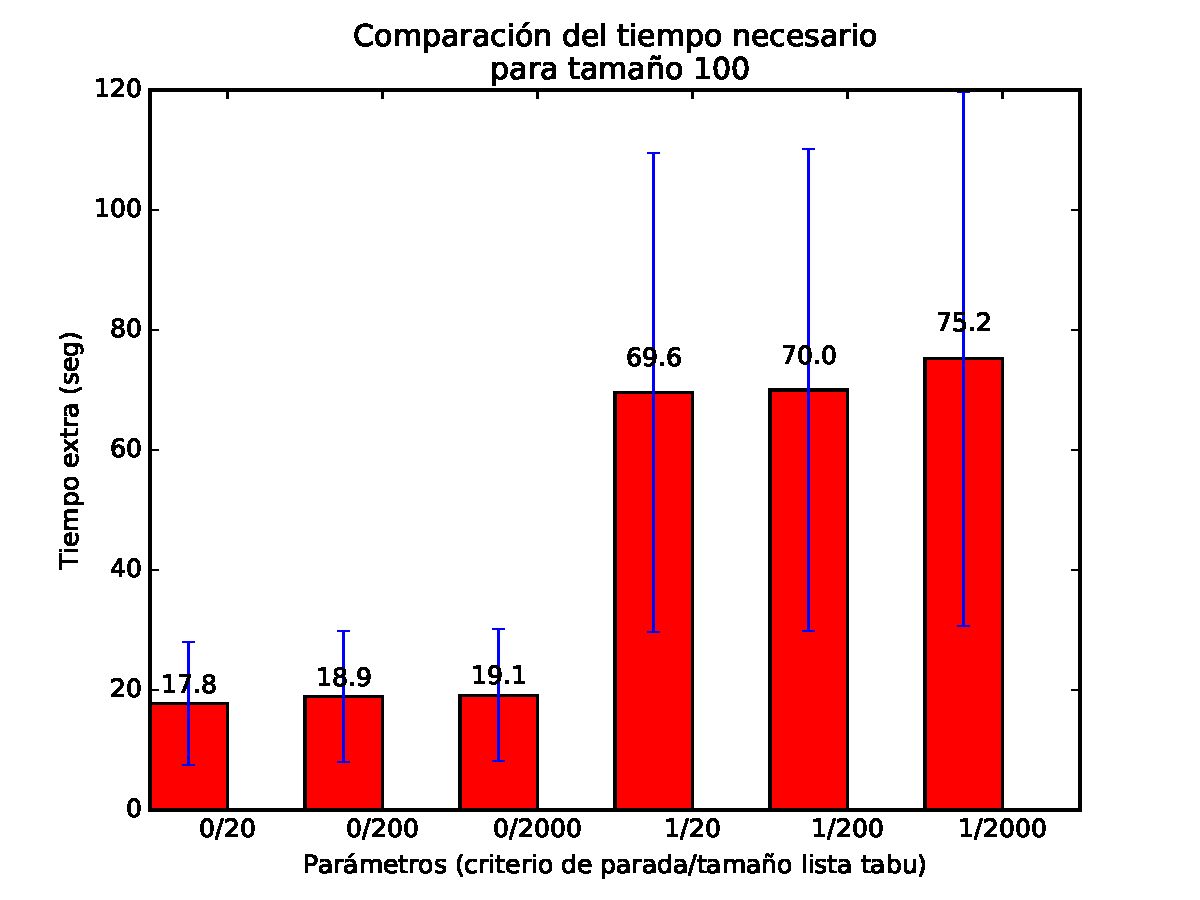
\includegraphics[width=0.8\textwidth]{graficos/problema_6/tiempo1.pdf}
	\caption{}
	\label{fig:problema6-tiempo1}
\end{figure}

\begin{figure}[H]
 \centering
	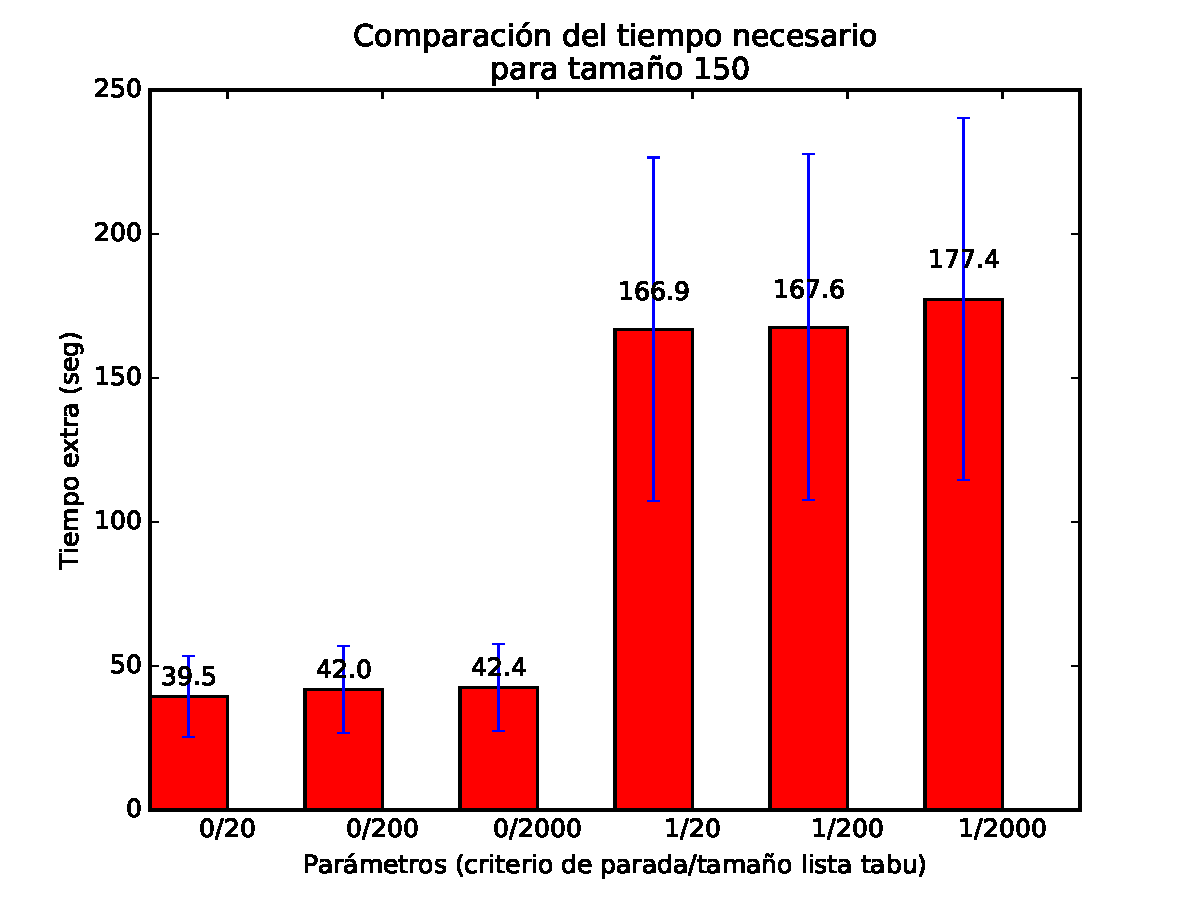
\includegraphics[width=0.8\textwidth]{graficos/problema_6/tiempo2.pdf}
	\caption{}
	\label{fig:problema6-tiempo2}
\end{figure}

En los gráficos se observa que confirmamos nuestras teorias de una manera bastante sólida.

Esto nos permite concluir que, aunque la calidad de las variantes es realmente similar, el tiempo que tardan los algoritmos es distinto, lo que nos permite concluir que la relación costo calidad de los algoritmos sí es diferente..

Esta relación costo calidad puede verse en los gráficos siguientes. En estos gráficos, dividimos la cantidad de aristas extra, sobre la el tiempo que tarda el algoritmo. Es decir, a más alto, mejor es el algoritmo.



%% COCIENTE

\begin{figure}[H]
 \centering
	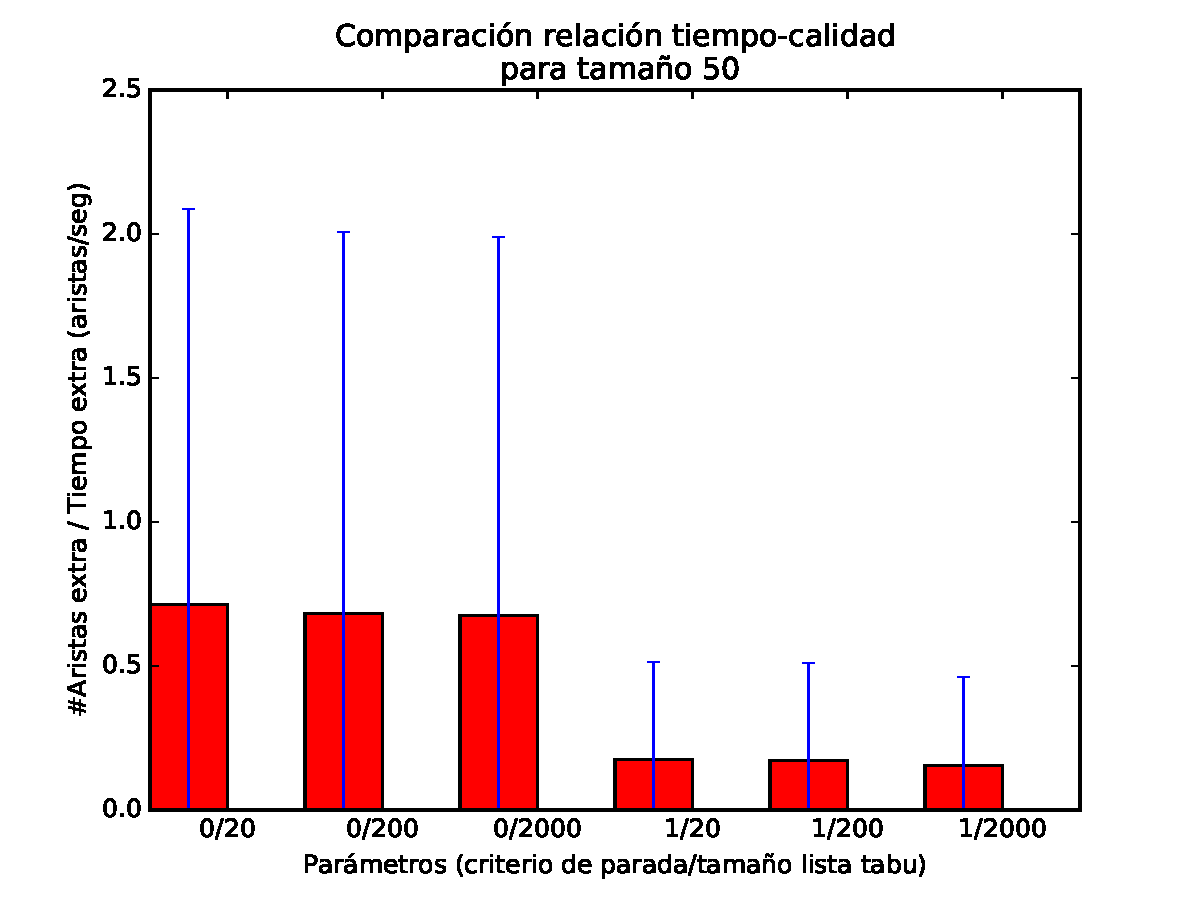
\includegraphics[width=0.8\textwidth]{graficos/problema_6/cociente0.pdf}
	\caption{}
	\label{fig:problema6-cociente0}
\end{figure}

\begin{figure}[H]
 \centering
	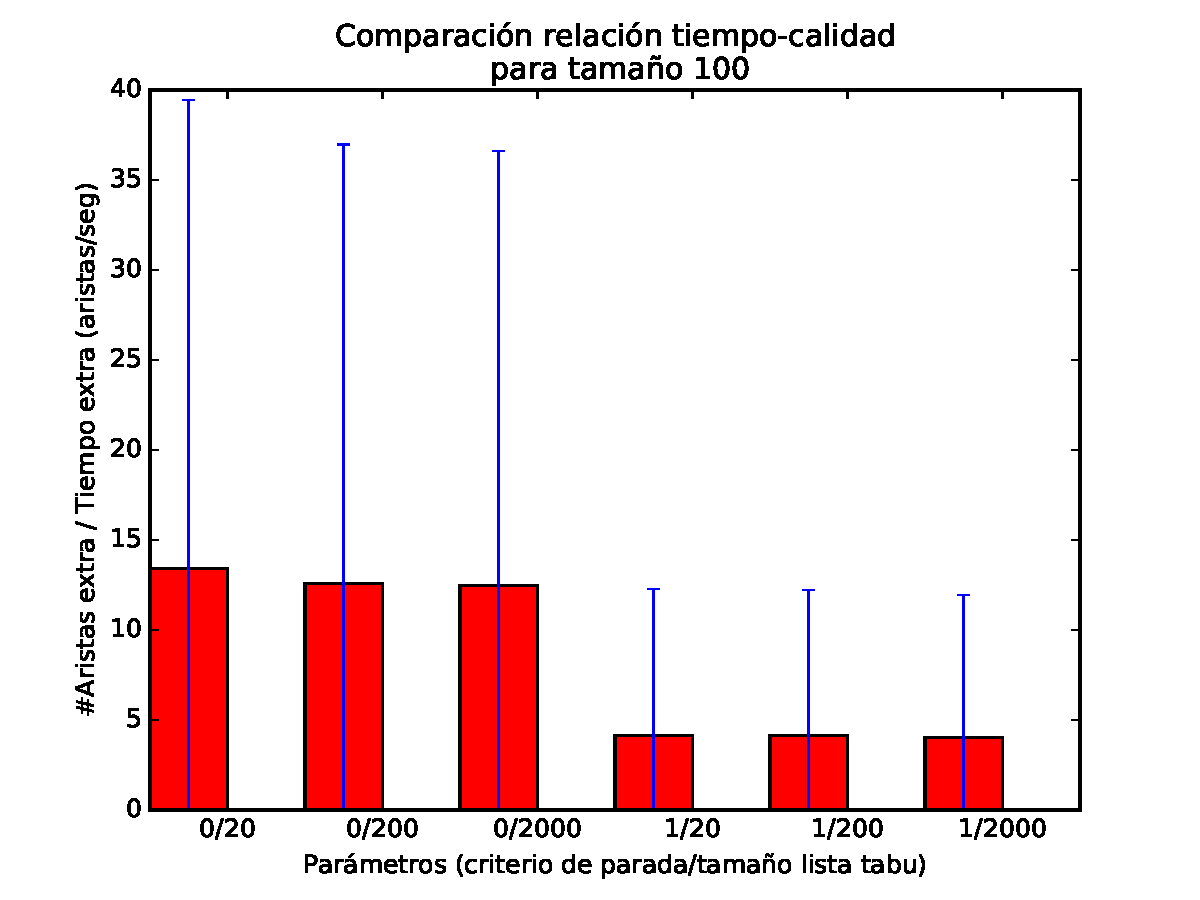
\includegraphics[width=0.8\textwidth]{graficos/problema_6/cociente1.pdf}
	\caption{}
	\label{fig:problema6-cociente1}
\end{figure}

\begin{figure}[H]
 \centering
	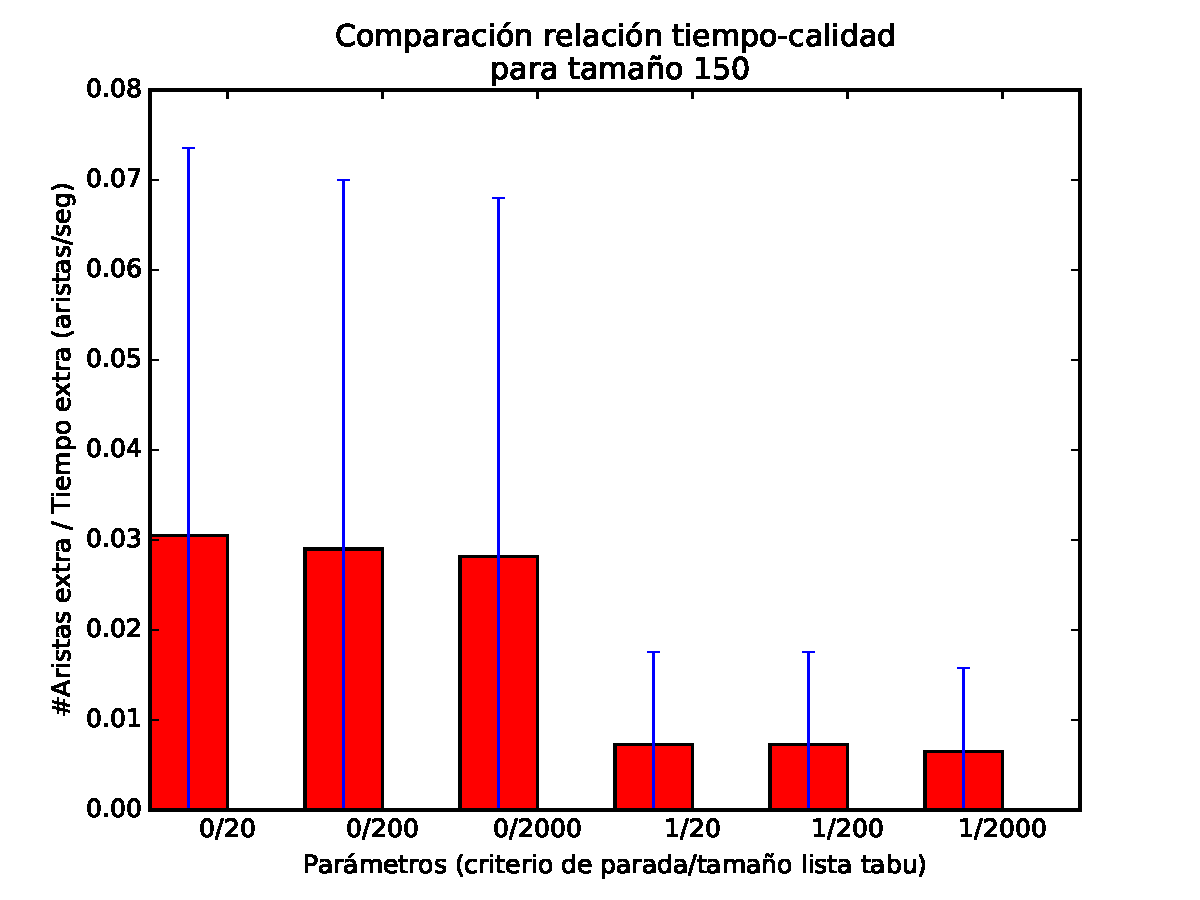
\includegraphics[width=0.8\textwidth]{graficos/problema_6/cociente2.pdf}
	\caption{}
	\label{fig:problema6-cociente2}
\end{figure}



